\documentclass{standalone}

\usepackage{xcolor}
%\definecolor{butter}{HTML}{FCE94F}
%\definecolor{butter}{HTML}{EDD400}
\definecolor{butter}{HTML}{C4A000}
%\definecolor{orange}{HTML}{FCAF3E}
%\definecolor{orange}{HTML}{F57900}
\definecolor{orange}{HTML}{CE5C00}
%\definecolor{chocolate}{HTML}{E9B96E}
%\definecolor{chocolate}{HTML}{C17D11}
\definecolor{chocolate}{HTML}{8F5902}
%\definecolor{chameleon}{HTML}{8AE234}
%\definecolor{chameleon}{HTML}{73D216}
\definecolor{chameleon}{HTML}{4E9A06}
%\definecolor{skyblue}{HTML}{729FCF}
%\definecolor{skyblue}{HTML}{3465A4}
\definecolor{skyblue}{HTML}{204A87}
%\definecolor{plum}{HTML}{AD7FA8}
%\definecolor{plum}{HTML}{75507B}
\definecolor{plum}{HTML}{5C3566}
%\definecolor{scarletred}{HTML}{EF2929}
%\definecolor{scarletred}{HTML}{CC0000}
\definecolor{scarletred}{HTML}{A40000}
%\definecolor{lightalu}{HTML}{EEEEEC}
%\definecolor{lightalu}{HTML}{D3D7CF}
\definecolor{lightalu}{HTML}{BABDB6}
%\definecolor{darkalu}{HTML}{888A85}
%\definecolor{darkalu}{HTML}{555753}
\definecolor{darkalu}{HTML}{2E3436}

\newcommand{\kwstyle}{}

\usepackage{listings}

\lstset{
%	backgroundcolor=\color{},
	basicstyle=\small\ttfamily\color{black},
%	breakatwhitespace=false,
	breaklines=true,
%	captionpos=b,
	commentstyle=\color{darkalu},
%	deletekeywords={...},
%	escapeinside={\%*}{*)},
%	extendedchars=true,
%	frame=single,
%	keepspaces=true,
	keywordstyle=\kwstyle,
	language=Caml,
%	morekeywords={*,...},
%	numbers=left,
%	numbersep=5pt,
%	numberstyle=\color{},
%	rulecolor=\color{},
%	showspaces=false,
%	showstringspaces=false,
%	showtabs=false,
%	stepnumber=2,
	stringstyle=\color{plum},
	tabsize=2,
%	title=\lstname,
	keywordstyle=[1]\kwstyle\color{chameleon},
	keywordstyle=[2]\kwstyle\color{scarletred},
	keywordstyle=[3]\kwstyle\color{skyblue},
	keywordstyle=[4]\kwstyle\color{butter},
	keywordstyle=[5]\kwstyle\color{skyblue},
	keywordstyle=[6]\kwstyle\color{skyblue},
	keywordstyle=[7]\kwstyle\color{chameleon},
	keywordstyle=[8]\kwstyle\color{butter},
	keywordstyle=[9]\kwstyle\color{butter},
	keywords=[1]{let,val,method,in,and,rec,private,virtual,constraint},
	keywords=[2]{type,open,class,module,exception,external},
	keywords=[3]{fun,function,functor,match,try,with},
	keywords=[4]{as,when,of},
	keywords=[5]{if,then,else},
	keywords=[6]{begin,end,object,struct,sig,for,while,do,done,to,downto},
	keywords=[7]{true,false},
	keywords=[8]{include,inherit,initializer},
	keywords=[9]{new,ref,mutable,lazy,assert,raise},
}

\lstset{literate=
	{0}{{{\kwstyle\color{plum}0}}}1 {0.}{{{\kwstyle\color{plum}0.}}}2
	{1}{{{\kwstyle\color{plum}1}}}1 {1.}{{{\kwstyle\color{plum}1.}}}2
	{2}{{{\kwstyle\color{plum}2}}}1 {2.}{{{\kwstyle\color{plum}2.}}}2
	{3}{{{\kwstyle\color{plum}3}}}1 {3.}{{{\kwstyle\color{plum}3.}}}2
	{4}{{{\kwstyle\color{plum}4}}}1 {4.}{{{\kwstyle\color{plum}4.}}}2
	{5}{{{\kwstyle\color{plum}5}}}1 {5.}{{{\kwstyle\color{plum}5.}}}2
	{6}{{{\kwstyle\color{plum}6}}}1 {6.}{{{\kwstyle\color{plum}6.}}}2
	{7}{{{\kwstyle\color{plum}7}}}1 {7.}{{{\kwstyle\color{plum}7.}}}2
	{8}{{{\kwstyle\color{plum}8}}}1 {8.}{{{\kwstyle\color{plum}8.}}}2
	{9}{{{\kwstyle\color{plum}9}}}1 {9.}{{{\kwstyle\color{plum}9.}}}2
	{->}{{{\kwstyle\color{chameleon}$\rightarrow$}}}2
}


\usepackage{tikz}
\usetikzlibrary[arrows]

\begin{document}
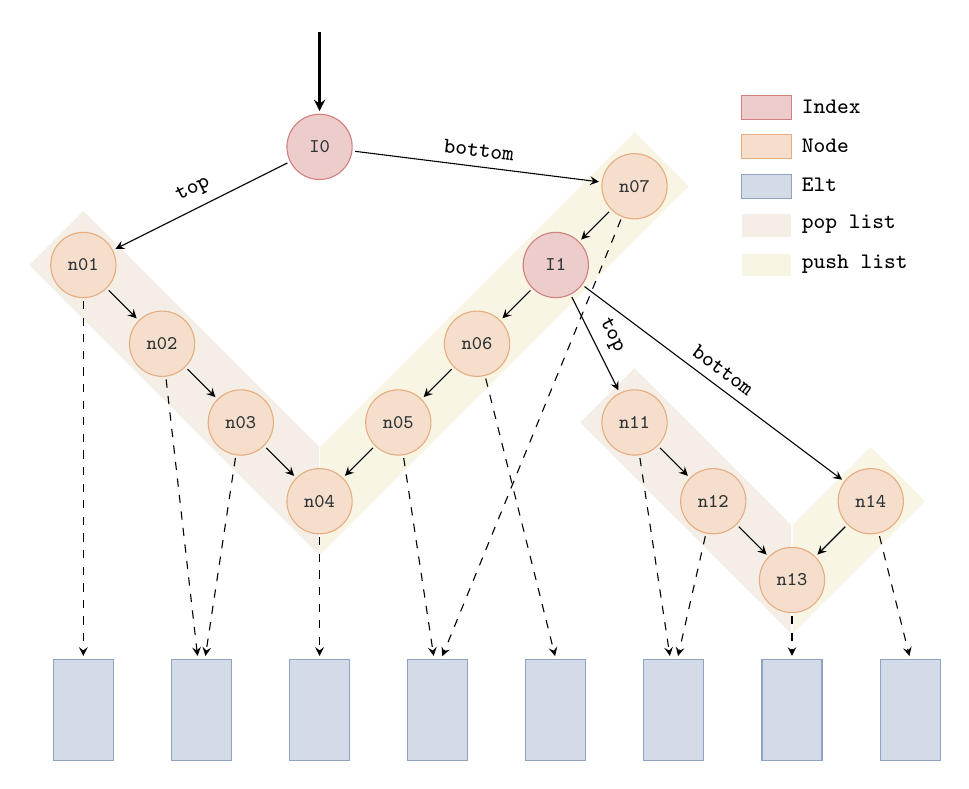
\begin{tikzpicture}[align=center,node distance=4em]

%\draw[step=1cm] (-10,-10) grid (10, 10);

\tikzstyle{txt}=[
	text width=2em,
	color=darkalu
]
\tikzstyle{index}=[
	text width=1em,
	text height=1em,
	circle,
	draw=scarletred!50,
	fill=scarletred!20
]
\tikzstyle{node}=[
	text width=1em,
	text height=1em,
	circle,
	draw=orange!50,
	fill=orange!20
]
\tikzstyle{elt}=[
	text width=1.5em,
	text height=3em,
	anchor=north,
	rectangle,
	draw=skyblue!50,
	fill= skyblue!20
]
\tikzstyle{lbox}=[
	text width=0.4cm,
	text height=0.2em,
	rectangle,
	anchor=east
]
\tikzstyle{ltxt}=[
	text height=0.4em,
	rectangle,
	anchor=west
]
\tikzstyle{arr}=[->, >=stealth, shorten <=1pt, shorten >=1pt]
\tikzstyle{arrelt}=[arr, dashed]

\draw[fill=chocolate!10, draw=white]
	(-3, 3.7) -- (0, 0.7) -- (0, -0.7) -- (-3.7, 3) -- cycle;
\draw[fill=butter!10, draw=white]
	(4, 4.7) -- (0, 0.7) -- (0, -0.7) -- (4.7, 4) -- cycle;

\draw[fill=chocolate!10, draw=white]
	(4, 1.7) -- (6, -0.3) -- (6, -1.7) -- (3.3, 1) -- cycle;
\draw[fill=butter!10, draw=white]
	(7, 0.7) -- (6, -0.3) -- (6, -1.7) -- (7.7, 0) -- cycle;

\coordinate (root) at (0, 6);
\node[index] (index) at (0, 4.5) {};
\draw[arr, thick] (root) -> (index);
\node[txt] at (0, 4.5) {\scriptsize\ttfamily I0};

\node[node] (n01) at (-3, 3) {};
\node[txt] at (-3, 3) {\scriptsize\ttfamily n01};
\node[node] (n02) at (-2, 2) {};
\node[txt] at (-2, 2) {\scriptsize\ttfamily n02};
\node[node] (n03) at (-1, 1) {};
\node[txt] at (-1, 1) {\scriptsize\ttfamily n03};
\node[node] (n04) at (0, 0) {};
\node[txt] at (0, 0) {\scriptsize\ttfamily n04};
\node[node] (n05) at (1, 1) {};
\node[txt] at (1, 1) {\scriptsize\ttfamily n05};
\node[node] (n06) at (2, 2) {};
\node[txt] at (2, 2) {\scriptsize\ttfamily n06};
\node[node] (n07) at (4, 4) {};
\node[txt] at (4, 4) {\scriptsize\ttfamily n07};

\node[index] (branch) at (3, 3) {};
\node[txt] at (3, 3) {\scriptsize\ttfamily I1};

\node[node] (n11) at (4, 1) {};
\node[txt] at (4, 1) {\scriptsize\ttfamily n11};
\node[node] (n12) at (5, 0) {};
\node[txt] at (5, 0) {\scriptsize\ttfamily n12};
\node[node] (n13) at (6, -1) {};
\node[txt] at (6, -1) {\scriptsize\ttfamily n13};
\node[node] (n14) at (7, 0) {};
\node[txt] at (7, 0) {\scriptsize\ttfamily n14};

\draw[arr] (index) -> (n01) node[sloped, midway, above]
	{\footnotesize\ttfamily top};
\draw[arr] (index) -> (n07) node[sloped, midway, above]
	{\footnotesize\ttfamily bottom};

\draw[arr] (branch) -> (n11) node[sloped, midway, above]
	{\footnotesize\ttfamily top};
\draw[arr] (branch) -> (n14) node[sloped, midway, above]
	{\footnotesize\ttfamily bottom};

\draw[arr] (n01) -> (n02);
\draw[arr] (n02) -> (n03);
\draw[arr] (n03) -> (n04);

\draw[arr] (n07) -> (branch);
\draw[arr] (branch) -> (n06);
\draw[arr] (n06) -> (n05);
\draw[arr] (n05) -> (n04);

\draw[arr] (n11) -> (n12);
\draw[arr] (n12) -> (n13);
\draw[arr] (n14) -> (n13);

\node[elt] (elt0) at (-3, -2) {};
\node[elt] (elt1) at (-1.5, -2) {};
\node[elt] (elt2) at (0, -2) {};
\node[elt] (elt3) at (1.5, -2) {};
\node[elt] (elt4) at (3, -2) {};
\node[elt] (elt5) at (4.5, -2) {};
\node[elt] (elt6) at (6, -2) {};
\node[elt] (elt7) at (7.5, -2) {};

\draw[arrelt] (n01) -> (elt0.north);
\draw[arrelt] (n02) -> (elt1.94);
\draw[arrelt] (n03) -> (elt1.86);
\draw[arrelt] (n04) -> (elt2.north);
\draw[arrelt] (n05) -> (elt3.94);
\draw[arrelt] (n06) -> (elt4.north);
\draw[arrelt] (n07) -> (elt3.86);
\draw[arrelt] (n11) -> (elt5.94);
\draw[arrelt] (n12) -> (elt5.86);
\draw[arrelt] (n13) -> (elt6.north);
\draw[arrelt] (n14) -> (elt7.north);

\node[lbox, draw=scarletred!50, fill=scarletred!20] at (6, 5) {};
\node[ltxt] at (6, 5) {\footnotesize\ttfamily Index};
\node[lbox, draw=orange!50, fill=orange!20] at (6, 4.5) {};
\node[ltxt] at (6, 4.5) {\footnotesize\ttfamily Node};
\node[lbox, draw=skyblue!50, fill=skyblue!20] at (6, 4) {};
\node[ltxt] at (6, 4) {\footnotesize\ttfamily Elt};
\node[lbox, draw=white, fill=chocolate!10] at (6, 3.5) {};
\node[ltxt] at (6, 3.5) {\footnotesize\ttfamily pop list};
\node[lbox, draw=white, fill=butter!10] at (6, 3) {};
\node[ltxt] at (6, 3) {\footnotesize\ttfamily push list};

\end{tikzpicture}
\end{document}